\section{Speciell relativitet}

\paragraph{Galileitransformationen}
Betrakta en statisk ram $S$ och en ram $S'$ som rör sig med konstant hastighet $\vb{u}$. Galileitransformen är den klassiska transformen av hastigheter och accelerationer mellan dessa system och ger
\begin{align*}
	\vb{r} = \vb{u}t + \vb{r}', \\
	\vb{v} = \vb{u} + \vb{v}', \\
	\vb{a} = \vb{a}'. \\
\end{align*}

\paragraph{Michelson-Morleys experiment}
Michelson-Morleys experiment visade att ljus omöjligt kunde propageras genom den postulerade etern.

Uppställningen som användes är (en mer avancerad variant av) Michelson-Morley-interferometern, som illustreras i figur \ref{fig:interferometer}.
\begin{figure}[!ht]
	\centering
	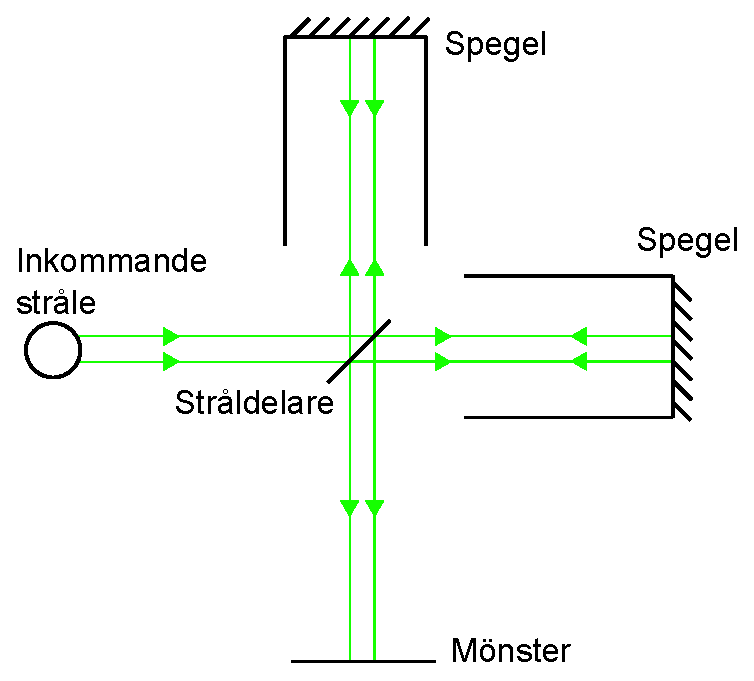
\includegraphics[width = 0.5\textwidth]{./Images/interferometer.eps}
	\caption{}
	\label{fig:interferometer}
\end{figure}

Ideen bakom experimentet var att de två "armarna" i uppställningen skulle röra sig med olika hastigheter relativt etern eftersom Jorden rör sig relativt Solen.

Om nu varje arm har längd $L$ och etern rör sig med en hastighet $u$ åt höger, tar ljuset tiden
\begin{align*}
	t_{\text{höger}} &= \frac{L}{c + u} + \frac{L}{c - u} \\
	                 &= L\frac{c - u + c + u}{c^{2} - u^{2}} \\
	                 &= \frac{2cL}{c^{2} - u^{2}} \\
	                 &= \frac{2L}{c}\frac{1}{1 - \frac{u^{2}}{c^{2}}}
\end{align*}
att röra sig till och från stråldelaren åt höger och tiden
\begin{align*}
	t_{\text{upp}} &= \frac{2L}{\sqrt{c^{2} - u^{2}}} \\
	               &= \frac{2L}{c}\frac{\sqrt{1 - \frac{u^{2}}{c^{2}}}}{1 - \frac{u^{2}}{c^{2}}},
\end{align*}
ty ljuset måste röra sig uppåt och motriktad hastigheten mot höger för att återvända till samma position i stråldelaren. Alltså borde skillnaden mellan tiden det tar för ljuset att röra sig de två vägarna ges av
\begin{align*}
	\Delta t = \frac{2L}{c}\frac{1 - \sqrt{1 - \frac{u^{2}}{c^{2}}}}{1 - \frac{u^{2}}{c^{2}}}.
\end{align*}
För Michelson och Morleys fal förutspådde de att de skulle se $0.4$ fransar i interferensmönstret, men de observerade $< 0.01$ fransar. Efter att ha upprepat sitt experiment ett halvår senare för att utesluta påverkan från Jordens position, konkluderade de med att det inte kunde finnas någon eter.

\paragraph{Einsteins postulat}
Baserad på Michelson-Morleys experiment, kom Einstein med följande postulat:
\begin{itemize}
	\item Fysikens lagar är de samma i alla inertialsystem.
	\item Ljushastigheten i vakuum har samma värde $c$ i alla inertialsystem.
\end{itemize}

\paragraph{Lorentztransformationen}
Lorentztransformationen är en transformation för att byta mellan olika referensramer. Den skiljer sig från Galileitransformationer, som inte är tillräcklig för att beskriva denna nya fysiken.

För att härleda Lorentztransformationen, betrakta två referensramar som sammanfallar vid $t = 0$ där den ena rör sig med en hastighet $v$ i $x$-riktning. För att beskriva transformationen, ansätter vi
\begin{align*}
	x' = k_{i}x_{i},
\end{align*}
där det summeras över alla rymdliga koordinater och tiden. Vi ansätter linjaritet eftersom det annars skulle kunna uppkomma accelererande rörelse i ett system utan att det är acceleration i ett annat, vilket skulle vara konstigt. Vidare antar vi att $x'$ ej beror av andra rymdliga kordinater, men att den kan bero av origos rörelse, och ansätter
\begin{align*}
	x' = k_{1}(x - vt).
\end{align*}
Antag nu att vi skickar ut en ljuspuls från origo vid $t = 0$. Vågfrontens avstånd från origo kommer beskrivas av
\begin{align*}
	x^{2} + y^{2} + z^{2} = c^{2}t^{2},
	x'^{2} + y^{2} + z^{2} = c^{2}t'^{2},
\end{align*}
eftersom ljuset skall ha samma fart i båda referensramer. Vi använder nu våran ansats för att transformera den andra ekvationen tillbaka, och får
\begin{align*}
	k_{1}^{2}x^{2} + y^{2} + z^{2} + k_{1}^{2}(v^{2}t^{2} - 2xvt) = c^{2}t'^{2}.
\end{align*}
Om vi sätter $t = t'$, får vi nu andra termer, och transformationen mislyckades. Vi åtgärder detta vid att ansätta
\begin{align*}
	t' = k_{t, 1}x + k_{t, 2}t.
\end{align*}
Detta ger
\begin{align*}
	k_{1}^{2}x^{2} + y^{2} + z^{2} + k_{1}^{2}(v^{2}t^{2} - 2xvt) = c^{2}(k_{t, 1}^{2}x^{2} + k_{t, 2}^{2}t^{2} + 2k_{t, 1}k_{t, 2}xt).
\end{align*}
För att transformationen skall lyckas, ger detta
\begin{align*}
	k_{1}^{2} - c^{2}k_{t, 1}^{2} = 1, \\
	vk_{1}^{2} + k_{t, 1}k_{t, 2}c^{2} = 0, \\
	c^{2}k_{t, 2}^{2} - k_{1}^{2}v^{2} = 0.
\end{align*}
Vid att införa
\begin{align*}
	\beta = \frac{v}{c}, \gamma = \frac{1}{\sqrt{1 - \beta^{2}}}
\end{align*}
kan lösningarna skrivas som
\begin{align*}
	k_{1} = k_{t, 2} = \gamma, k_{t, 1} = -\frac{\beta\gamma}{c}.
\end{align*}
Lorentztransformationerna ges då av
\begin{align*}
	x' = \gamma(x - vt), t' = \gamma\left(t - \frac{\beta}{c}x\right).
\end{align*}
Den inversa Lorentztransformationen fås vid att lösa ut ekvationerna för $x$ och $t$, och ges av
\begin{align*}
	x = \gamma(x' + vt'), t = \gamma(t' + \frac{\beta}{c}x').
\end{align*}
Med de givna skalfaktorerna ser vi att för små hastigheter går detta över i Galileitransformer, medan inga hastigheter över $c$ tillåts.

\paragraph{Samtidighet}
Betrakta två händelser som inträffer vid olika tidspunkter och positioner. Lorentztransformationen ger
\begin{align*}
	\Delta t = \gamma(\Delta t' + \frac{\beta}{c}\Delta x').
\end{align*}
Detta implicerar att om händelserna är samtidiga i en referensram, är de inte nödvändigtvis det i den andra.

\paragraph{Tidsdilation}
Betrakta två händelser som inträffer vid samma position i den rörliga ramen. Lorentztransformationen ger
\begin{align*}
	\Delta t = \gamma\Delta t',
\end{align*}
och det mäts en längre tidsskilland mellan händelserna i inertialramen.

\paragraph{Längdkontraktion}
Betrakta två händelser som inträffer vid samma tidspunkt i inertialramen. Lorentztransformationen ger
\begin{align*}
	\Delta x = \frac{1}{\gamma}\Delta x,
\end{align*}
och det mäts ett kortare avstånd mellan händelserna i inertialramen.